\chapter{Analysis}

\section {Instruction Pipelining}
\subsection {Introduction}
In the 1970s and 1980s in response to the increasing complexity of CISC(Complex Instruction Set Computer) processors researchers realized that simplifying the instruction set could lead to better performance. This insight is how the first RISC(Reduced Instruction Set Computer) projects were developed\cite{aletan1992overview}.
And almost simultaneously, the concept of pipelining was introduced. Pipelining is a method used to enhance a processor's throughput by overlapping the execution phases of multiple instructions. By dividing the execution of an instruction into several stages and executing multiple instructions concurrently, the processor can handle several instructions simultaneously, thereby increasing its throughput\cite{olanrewaju2017design}. Figure \ref{fig:pipeline} illustrates the concept of pipelining.
\begin{figure}[H]
    \centering
    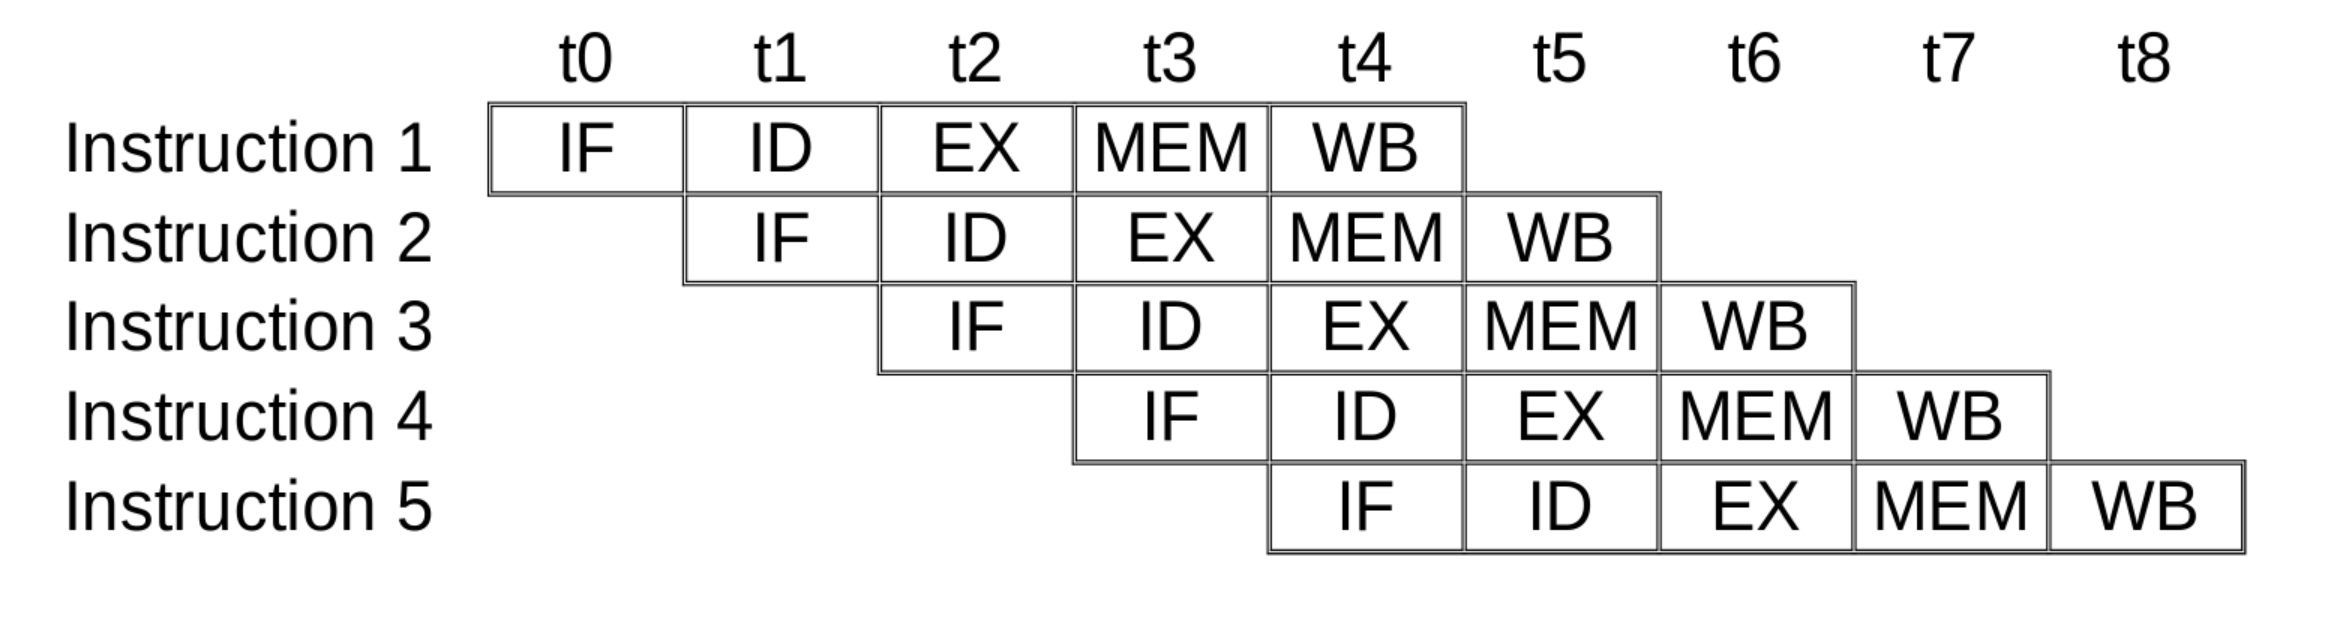
\includegraphics[width=0.8\textwidth]{assets/images/pipeline.png}
    \caption{Pipelining}
    \label{fig:pipeline}
\end{figure}


\subsection {Instruction Pipeline Stages}
The classical RISC pipeline consists of five stages: instruction fetch, instruction decode, execute, memory access, and write-back \cite{enwiki:1255528196}. 

\begin{itemize}
     \item \textbf{Instruction Fetch (IF)}: Fetches the instruction from memory using the program counter, which is then incremented.
     \item \textbf{Instruction Decode (ID)}: Decodes the instruction to determine the operation and fetches operands from the register file.
     \item \textbf{Execute (EX)}: Performs the operation on the fetched operands.
     \item \textbf{Memory Access (MEM)}: Accesses memory for load/store instructions; otherwise, bypassed.
     \item \textbf{Write-back (WB)}: Writes the result back to the destination register.
\end{itemize}\cite{he2023survey}

\subsection {Pipeline Hazards}
A hazard is a condition that occurs when the pipeline cannot execute the next instruction in the cycle. There are three types of hazards: structural, data, and control hazards.\cite{olanrewaju2017design}
\subsubsection {Structural Hazards}
Structural hazards occur when the hardware cannot support the combination of instructions in the pipeline. For example, if two instructions require the same hardware resource, such as the memory unit\cite{pandey2016study}.
This stalls the pipeline or corrupts a result.\cite{proebsting1994detecting}
\subsubsection {Data Hazards}
Data hazards occur when an instruction depends on the result of a previous instruction. There are three types of data hazards: read-after-write (RAW), write-after-read (WAR), and write-after-write (WAW). 

\begin{itemize}
    \item \textbf{Read-After-Write (RAW)}: Occurs when an instruction reads a register before a previous instruction writes to it. 
    \begin{itemize}
        \item \textbf{Solution}: Use techniques such as forwarding (or bypassing), where we add extra paths to the pipeline to allow the result of an instruction to be forwarded to the next instruction that needs it.
    \end{itemize}
    \item \textbf{Write-After-Read (WAR)}: Occurs when an instruction writes to a register before a previous instruction reads from it.
    \begin{itemize}
        \item \textbf{Solution}: This hazard is rare in RISC architectures due to the use of register renaming, which ensures that each instruction has a unique destination register.
    \end{itemize}
    \item \textbf{Write-After-Write (WAW)}: Occurs when two instructions write to the same register.
    \begin{itemize}
        \item \textbf{Solution}: Similar to WAR hazards, register renaming can be used to avoid WAW hazards by ensuring that each write operation targets a unique register.
    \end{itemize}
\end{itemize}\cite{pandey2016study}

\subsubsection {Control Hazards}
Control hazards occur when the pipeline makes a decision based on a previous instruction that has not yet completed. For example, a branch instruction may change the program counter before the next instruction has been fetched. This can lead to incorrect execution of instructions.\cite{pandey2016study}

\subsection {Pipeline Stalls}
Pipeline stalls occur when the pipeline cannot proceed due to a hazard. Stalls can be resolved by inserting no-operation (NOP) instructions or by forwarding data to the next instruction. However, these solutions can reduce the performance of the pipeline.\cite{pandey2016study}

\subsection {Pipeline Performance Metrics}
There are several metrics used to evaluate the performance of a pipeline, including throughput, speedup, and efficiency.

\begin{itemize}
    \item \textbf{Throughput}: The number of instructions completed per unit of time.
    \item \textbf{Speedup}: The ratio of the execution time of a non-pipelined processor to the execution time of a pipelined processor.
    \item \textbf{Efficiency}: The ratio of the speedup to the number of pipeline stages.
    \item \textbf{IPC (Instructions Per Cycle)}: The average number of instructions executed per clock cycle.
    \item \textbf{CPI (Cycles Per Instruction)}: The average number of clock cycles required to execute an instruction.
    \item \textbf{Cycles Per Second (CPS)}: The number of clock cycles per second.
    \item \textbf{Clock Rate}: The frequency at which the processor operates.
    \item \textbf{Latency}: The time taken to complete a task.
    \item \textbf{Throughput}: The number of tasks completed per unit of time.
    \item \textbf{Bandwidth}: The amount of data that can be transferred in a given time.
    \item \textbf{Response Time}: The time taken to respond to a request.
\end{itemize}\cite{pandey2016study}


\section {Existing Solutions}
















